%chktex-file 46
%chktex-file 21
%chktex-file 3
%chktex-file 13
%chktex-file 8
%chktex-file 25

Concrete degradation is a factor to account for in the long-term performance assessment of radioactive waste disposals, considering their environmental exposure. Over time, degradation processes such as carbonation can lower the alkalinity of concrete, which is essential for protecting from corrosion the steel reinforcements within these structures.
The onset of corrosion can compromise the integrity of containment walls, potentially leading to breaches that could release radioactive contaminants into the environment, and ultimately dose intake.
Properly accounting for these degradation pathways in the performance assessment of radioactive waste repositories over climatic projections is essential for ensuring the containment's longevity and, hence, the protection of public health and the environment. By implementing an eBN, chemical degradation of concrete structures is here evaluated over climatic change projections. 

\subsection{Concrete degradation}
Two most critical degradation processes impacting concrete infrastructure in radioactive waste disposals are carbonation-induced corrosion and chloride-induced corrosion. This section provides a concise overview of both phenomena and presents their respective mathematical models.

\subsubsection{Carbonation-induced corrosion}\label{Carbonation_corrosion_Chpt}
The presence of $CO_2$ increases the risk of carbonation-induced corrosion in concrete structures~\cite{TALUKDAR_part1,TALUKDAR_part2}. 
The interaction between concrete and atmospheric $CO_2$ causes the formation of calcium carbonate, a process known as carbonation, which reduces the concrete's alkalinity and makes the steel reinforcement in the concrete susceptible to corrosion~\cite{GLASSER2008226}.
Carbonation is quantified by measuring the depth from the concrete surface to where the alkalinity reaches a minimum allowable value. 
Once carbonation reaches the steel reinforcements, the corrosion propagation phase begins, accelerating the degradation of the concrete structure.
In this study, the carbonation depth, denoted as $x_c(t)$, is assessed using the model of~\textcite{Carb_eq_STEWART,Carb_eq_BASTIDASARTEAGA}.
Specifically, Eq.\ref{3:carbonation_depth} describes the increment in carbonation depth $\Delta x_c$ at time $t$, relative to the depth reached at time $t-\Delta T$, where $\Delta T$ denotes the selected evaluation interval in years, e.g., for a decade, $\Delta T = 10$.
\begin{equation}
    \label{3:carbonation_depth}
    \Delta x_c(t, \Delta T) = \sqrt{\frac{2 \ k_{site} \ C_{CO_2}(t) \ f_T^C(t) \ f_{RH}^C(t) \ (D_0^C)^{-n_d}}{a} \ \Delta T} \ \cdot \ \left( \frac{1}{\tau (t, \Delta T)} \right)^{n_m} 
\end{equation}
In defining $\Delta x_c$, $\tau (t, \Delta T)$ is an integer representing the number of $\Delta T$ intervals needed from the reference year to reach the evaluation year $t$, e.g., $t = 2020$ implies $\tau = 1$, $t = 2030$ implies $\tau = 2$, and so on.
The variable $k_{site}$ accounts for potentially higher $CO_2$ concentration values in industrial and urban areas; $C_{CO_2}$ is the time-dependent $CO_2$ concentration measured in \si{\kilogram\per\cubic\meter} is the $CO_2$ diffusion coefficient at reference time $t_0$, measured in \si{\square\meter\per\second}; $n_d$ is the diffusion coefficient aging factor; and $n_m$ is a factor accounting for exposure to microclimatic wetting and drying cycles, with a value of $0$ for sheltered outdoor environments and $0.12$ for unsheltered outdoor. \\
The time-independent quantity $a$ is derived from Eq.\ref{eq_a}, where $\alpha_h$ is the degree of hydration, expressed as a function of the water-to-cement ratio $w / c$. The cement content $Ce$ is measured in \si{\kilogram\per\cubic\meter}, the calcium oxide fraction in cement $CaO$ is approximately 0.65, and the molar masses of $CO_2$ and $CaO$ are \SI{44}{\kilogram\per\mole} and \SI{56}{\kilogram\per\mole}, respectively.
\begin{equation}
    \left\{
    \begin{array}{ll}
    a = 0.75 \ Ce \ CaO \ \alpha_H \frac{M_{CO_2}}{M_{CaO}} \\
      \\
      \alpha_h = 1 - e^{-3.38 \frac{w}{c}}
    \end{array}
    \right.
    \label{eq_a}
\end{equation}
The time-dependent quantities $f_T^C$ and $f_{RH}^C$ allow the incorporation of climate variable effects, associated with climate change projections, into the carbonation depth evaluation, as presented in the analytical models by~\textcite{Carbonation_BASTIDASARTEAGA}. 
Specifically, $f_T^C$ represents the dynamic effect of temperature on carbonation, impacting the diffusion coefficient according to the Arrhenius Law~\cite{Carbonation_YOON}, as shown in Eq.\ref{3:ft}. Here, $E$ is the activation energy of the diffusion process, i.e.,
\SI{38.3}{\kilo\joule\per\mole}; $R$ is the gas constant, i.e., \SI{8.314}{\kilo\joule\per\mole\per\kelvin}; $T(t_0)$ is the reference temperature, i.e.,\SI{293}{\kelvin}; and $T(t)$ is the temperature in Kelvin at time $t$.
\begin{equation}
    \label{3:ft}
        f_T^C (t) = e^{\frac{E}{R} \left[ \frac{1}{T_0} - \frac{1}{T(t)} \right]}
\end{equation}
The effect of relative humidity (RH) has been extensively studied. Research by~\textcite{f_rh_Al-Khaiat} suggests that RH levels below 30\% do not significantly impact carbonation depth, whereas~\textcite{f_rh_BARY} indicates that RH levels above 50\% have a significant influence. For this study, the analytical model chosen to describe the RH effect over time on the diffusion coefficient is the one proposed by~\textcite{Carbonation_BASTIDASARTEAGA}, detailed in Eq.\ref{3:frh}.
\begin{equation}
    \left\{
    \begin{array}{ll}
    0 & if \ RH \leq 0.25\\
    \left[\frac{1-RH(t)^\beta}{1-RH_0^\beta} \right]^\alpha & otherwise
    \end{array}
    \right.
    \label{3:frh}
\end{equation}
Here, $RH_0$ is the reference value for RH, whereas $\alpha$ and $\beta$ are independent parameters of exposure conditions. In this case study, the reference RH is set to 0.65, $\alpha$ is 5 and $\beta$ is 2.5.

\subsubsection{Chloride-induced corrosion}\label{Chloride_corrosion_Chpt}
The penetration and movement of chloride ions into concrete structures involve the electrochemical dissolution of iron, leading to the degradation of concrete barriers.
Chloride ingress into concrete is typically described using a diffusion model, which is a single mass transport equation for chloride ion transport.
In this study, a time-dependent model is applied, incorporating the chloride diffusion coefficient to estimate chloride concentration over time. The chloride concentration at a depth $z$ and time $t$ is described by Eq.~\ref{eq:chloride_corrosion}.
\begin{equation}
    \label{eq:chloride_corrosion}
    C(z, t) = C_0^{Cl} \left[ 1-erf \left(\frac{z}{2\sqrt{k_e \ k_t \ k_c \ f_T^{Cl}(t) \ f_{RH}^{Cl}(t) \ D_0^{Cl} \ \omega \ \tau(t, \Delta T)}} \right) \right]
\end{equation}
Here, $C_0^{Cl}$ represents the chloride concentration at the boundary; for atmospheric areas remote from coasts, $C_0^{Cl}$ is typically around \SI{1.15}{\kilogram\per\cubic\meter}, whereas, in coastal or tidal areas, the chloride concentration at the surface is significantly higher. $D_0^{Cl}$ is the reference chloride diffusion coefficient; $k_e$ is the environmental coefficient; $k_t$ is the test method factor and $k_c$ is the curing factor. 
Coefficient $\omega$ represents the number of seconds in 10 years whereas $\tau(t, \Delta T)$ has the same definition given in Sec.~\ref{Carbonation_corrosion_Chpt}.\\
Similar to carbonation, there are two time-dependent quantities that account for the effects of climate change projections on temperature and relative humidity: $f_{T}^{Cl}$ and $f_{RH}^{Cl}$.
\begin{equation}
    \label{eq_f_rh_cl}
    f_{RH}^{Cl}(t) = \left[ 1 + \frac{(1-RH(t))^4}{(1-RH_0)^4} \right]^{-1}
\end{equation}
The temperature effect is consistent with that defined for carbonation in Eq.\ref{3:ft}, thus $f_T^C = f_T^{Cl}$. The effect of RH is expressed in the work of~\textcite{f_RH_ClELHASSAN} as shown in Eq.\ref{eq_f_rh_cl}.

\subsection{eBN for concrete degradation}
The eBN framework is exemplified to perform the analysis of concrete degradation considering climatic change projections. 
Climate change data are taken from the catalogue provided in~\textcite{Copernicus_Climate_Change} and include three main projection scenarios referred to three different Shared Socio-economic Pathways, namely \textit{ssp1}, \textit{ssp2} and \textit{ssp5}. 
These projections account for variations in temperature, $CO_2$ concentration and relative humidity from 2020 to 2100, relevant for concrete corrosion models.\\ 
In this study, the eBN integrates the two degradation models presented in~\ref{Carbonation_corrosion_Chpt} and in~\ref{Chloride_corrosion_Chpt}, and is structured to capture the probabilistic dependencies, considering epistemic and aleatoric uncertainties, between climate conditions of temperature, relative humidity and $CO_2$ concentration, material properties, e.g.~diffusion coefficients, water-to-cement ratio and the final state of the system, through the carbonation and chloride effects on concrete.
The following sections detail the eBN structure, the probabilistic modelling of the input variables and its application to the case study of concrete structures degradation in a radioactive waste disposal. 
Initially, the carbonation-induced and chloride-induced corrosion models are examined separately to enhance clarity and comprehensibility. 
Subsequently, the complete eBN framework, integrating both degradation mechanisms, is presented.

\subsubsection{eBN -- Carbonation-induced corrosion model}\label{ebn_carbonation_section}
The eBN representing the carbonation process, illustrated in Fig.~\ref{carbonation_ebn}, includes two primary discrete root nodes. The first is the node \textit{t}, which denotes the selected time slice (considering $\Delta T$ equals to a decade); it consists of nine equally probable states, corresponding to the decades from 2020 to 2100. The second node, \textit{proj}, represents the climate change projections, with three equally likely states, each associated with an \textit{ssp} (i.e~\textit{ssp1}, \textit{ssp2} and \textit{ssp5}).
\begin{figure}[H]
    \centering
    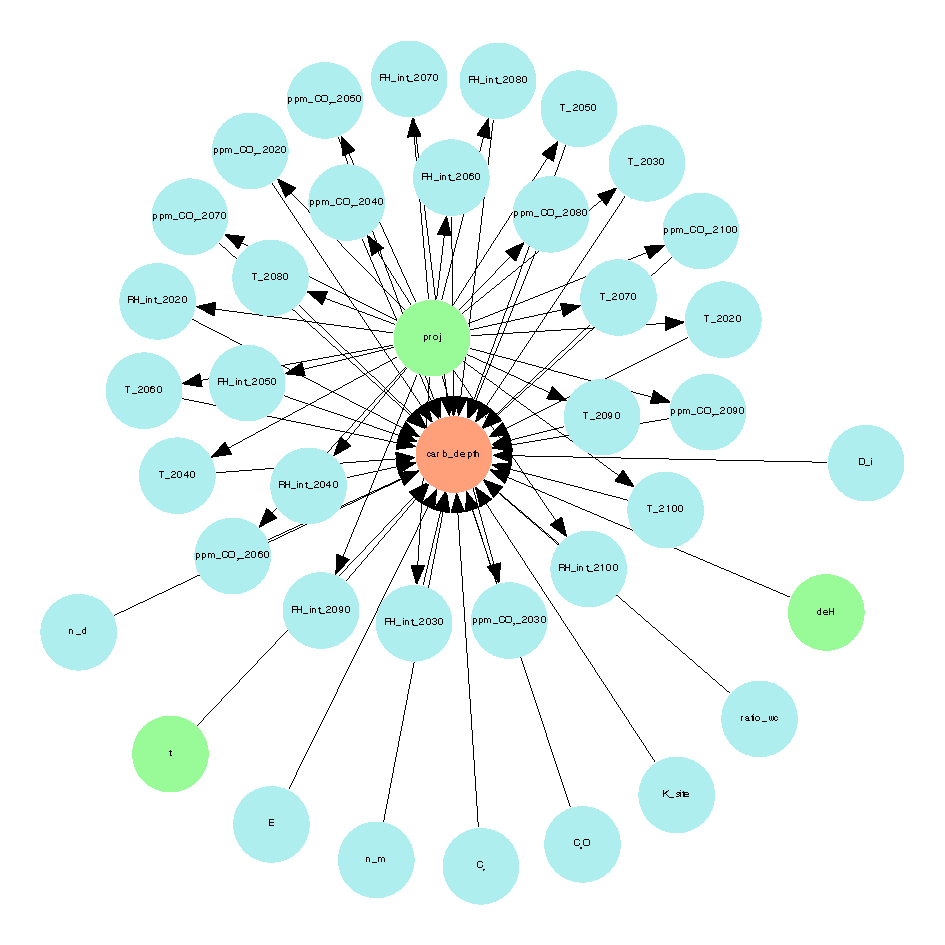
\includegraphics[width=\linewidth]{imgs/pdfs/8_carb_ebn.pdf}
    \caption{Carbonation-induced corrosion eBN with precise nodes}\label{carbonation_ebn}
\end{figure}
A third discrete root node, \textit{DeH}, is also shown in Fig.~\ref{carbonation_ebn}. This node represents a control variable to reduce the RH below a threshold. Specifically, whenever RH exceeds 0.25, the node enforces a reduction to 0.2. These values were selected based on the influence of RH on the carbonation model, as illustrated in Fig.~\ref{carbonation_depth vs RH}.
\begin{figure}[H]
    \centering
    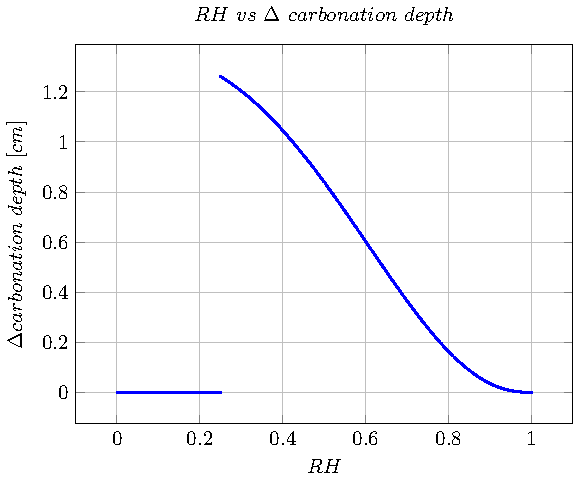
\includegraphics[scale=0.7]{imgs/pdfs/10_RH_carb.pdf}
    \caption{RH effect on carbonation depth}\label{carbonation_depth vs RH}
\end{figure}
The \textit{DeH} node is modelled as a Boolean variable with two states: failed ($P_{F} = 10^{-4}$) and working ($P_{W} = 1 - 10^{-4}$). \\
In addition, eight continuous root nodes are introduced to account for aleatoric uncertainties in the parameters $n_d$, $n_m$, $E$, $k_{site}$, water-to-cement ratio ($w/c$), $C_e$, $CaO$ and $D_0^C$. Their CPTs are provided in Table~\ref{continuous_root_node_ebn_carb}.
\begin{table}[hbt!]
    \begin{center}
        \caption{Distribution of the continuous root nodes of the eBN depicted in Fig.\ref{carbonation_ebn}}\label{continuous_root_node_ebn_carb}
        \begin{tabular}{P{2cm}P{2.2cm}P{6cm}}
            \textbf{Quantity} & \textbf{Node Name} & \textbf{Distribution} \\
            \midrule
            $n_d$       & $n \_ d$          & $Trunc(N(0.24;2.88e^{-2}); 0, \infty)$ \\
            $n_m$       & $n \_ m$          & $Trunc(N(0.12;1.2e^{-2}); 0, \infty)$\\
            $E$         & $E$               & $Uniform(34.853;41.747)$ \\
            $k_{site}$  & $k \_ site$       & $Trunc(N(1.15;1.15e^{-2}); 0, \infty)$ \\
            $w / c$     & $ratio \_ w/c$    & $Trunc(LogN(-0.69; 0.05); 0, 1)$ \\
            $Ce$        & $C_e$             & $Trunc(N(300;30); 0, \infty)$ \\
            $CaO$       & $C_aO$            & $Uniform(0.585; 0.715)$ \\
            $D_0^C$     & $D \_ i$          & $Trunc(N(2.2e^{-4};1.5e^{-5}); 0, \infty)$ \\
        \end{tabular}
    \end{center}
\end{table}
The carbonation process is governed by the model presented in Eq.~\ref{3:carbonation_depth}, which explicitly depends on temperature, $CO_2$ concentration and RH. 
These variables are characterized through climate change projections data for a nuclear waste disposal located in Belgium (see Appendix~\ref{appendixA}). \\
The model is dynamic in nature, as its output corresponds to the increment in carbonation depth accumulated over the decade ending in the year under consideration. Therefore, to evaluate the total carbonation depth, one must consider the cumulative sum of increments from all preceding decades.
We have introduced decade-specific nodes for temperature, $CO_2$ concentration (in ppm) and relative humidity over decades.
Examples include $T\_ {2020}$, $T\_ {2030}$ and so on up to $T\_ {2100}$, as shown in Fig.~\ref{carbonation_ebn}. These nodes are all modelled as children of the \textit{proj} node, with distributions detailed in Tables~\ref{Climate_Change_Tnode_dists},~\ref{Climate_Change_RHnode_dists} and~\ref{Climate_Change_CO2node_dists}.
This structure supports the definition of the functional node \textit{carb\_depth}, which is a child of all temperature, $CO_2$ and RH nodes, as well as of \textit{proj}, \textit{DeH} and the time slice node \textit{t}. 
For each time slice, a dedicated model computes the incremental carbonation depth by summing contributions from previous decades. 
If the resulting total exceeds the threshold of 3 cm, defined by~\textcite{Carbonation_BASTIDASARTEAGA}, the system transitions to a failure state. 
In the carbonation model, the inputs from the $ratio\_w/c$ node and all the RH percentage change nodes are modified before being passed to the computational component. 
Specifically, the $ratio\_w/c$ samples are scaled by a factor of 0.1 and then shifted by +0.5, whereas the RH percentage change samples are randomly assigned as either positive or negative deviations from the reference RH.

\subsubsection{eBN -- Chloride-induced corrosion model}\label{ebn_chloride_section}
The chloride-induced corrosion process is represented by the eBN depicted in Fig.~\ref{chloride_ebn}. This model includes some of the same continuous nodes as the corrosion process eBN, specifically for temperature, $CO_2$ concentration, RH. It also shares the  discrete nodes \textit{proj}, \textit{t} and \textit{DeH}. The effect of relative humidity on the chloride penetration is shown in Fig.~\ref{RH vs chloride depth}.
\begin{figure}[H]
    \centering
    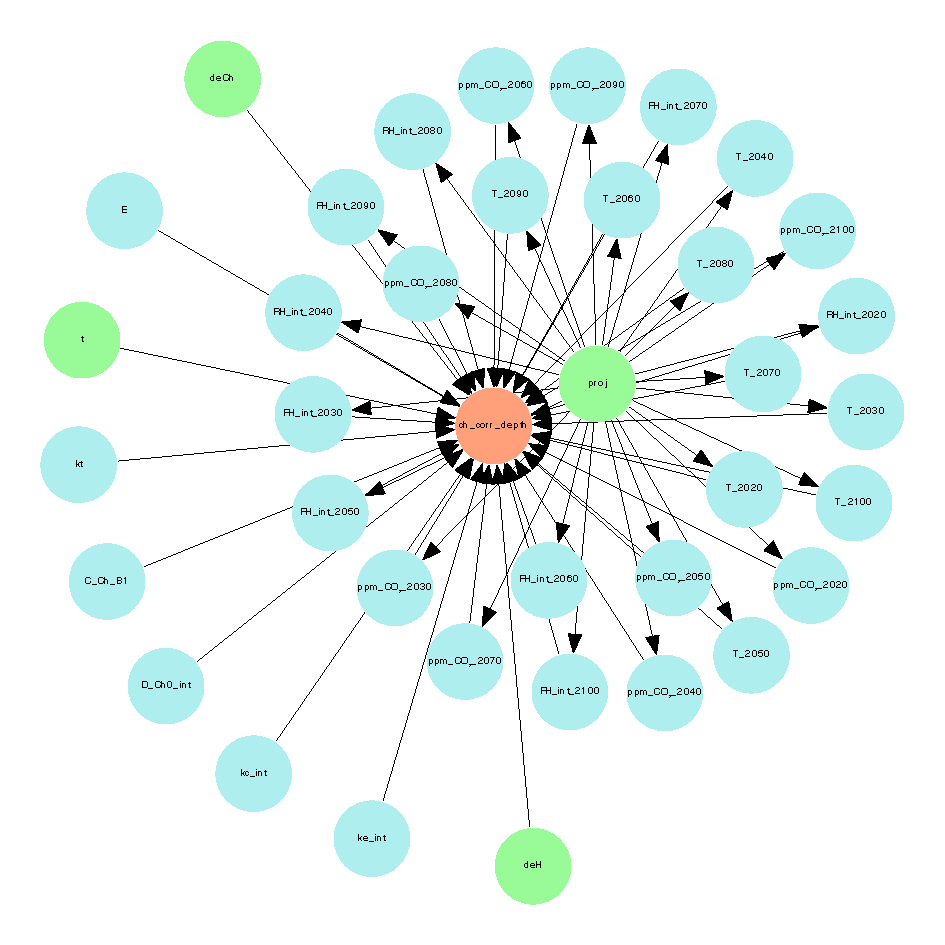
\includegraphics[width=\linewidth]{imgs/pdfs/9_chloride_ebn.pdf}
    \caption{Chloride-induced corrosion eBN with precise nodes}\label{chloride_ebn}
\end{figure}
\begin{figure}[H]
    \centering
    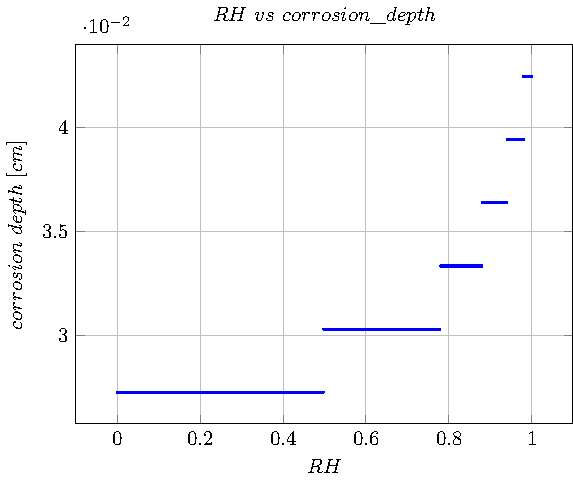
\includegraphics[scale=0.7]{imgs/pdfs/11_RH_corr.pdf}
    \caption{RH effect on chloride penetration depth}\label{RH vs chloride depth}
\end{figure}
\begin{figure}[H]
    \centering
    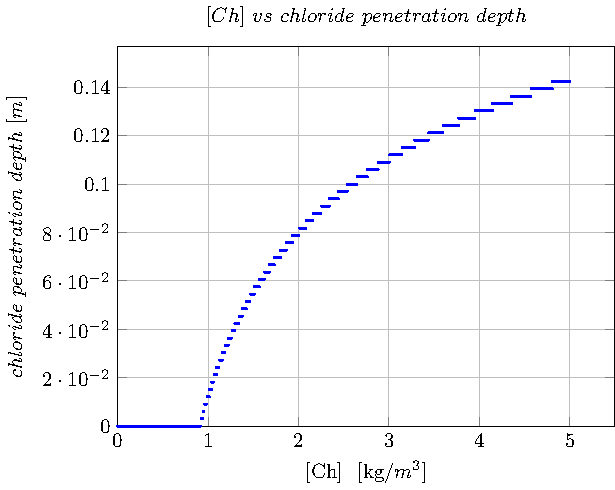
\includegraphics[scale=0.7]{imgs/pdfs/11_Chloride_corr.pdf}
    \caption{Chloride concentration at system boundary effect on chloride penetration depth}\label{Chloride vs corrosion depth}
\end{figure}

\textit{DeCh} is a discrete root node that represents a chloride mitigation control variable that reduces the boundary chloride concentration, $C_0^{Cl}$, when it exceeds a critical level.
The effect of the boundary chloride concentration on the model is shown in Fig.~\ref{Chloride vs corrosion depth}. $DeCh$ node is modelled as a Boolean variable with states \textit{working} and \textit{failed}, with assigned probabilities $P_W = 1 - 10^{-4}$ and $P_F = 10^{-4}$, respectively. It is designed to lower $C_0^{Cl}$ from values above 0.9 to 0.7. \\
Five continuous root nodes are also included to represent aleatoric uncertainties in the parameters $k_t$, $k_c$, $k_e$, $C_0^{Cl}$, and the reference diffusion coefficient $D_0^{Cl}$. Their distributions are detailed in Table~\ref{continuous_root_node_ebn_ch}.

\begin{table}[hbt!]
    \begin{center}
        \caption{Continuous root node distribution of the eBN in Fig.\ref{chloride_ebn}}\label{continuous_root_node_ebn_ch}
        \begin{tabular}{P{1.6cm}P{2.1cm}P{6cm}}
            \textbf{Quantity} & \textbf{Node Name} & \textbf{Distribution} \\
            \midrule
            $k_t$       & $kt \_ int$      & $Trunc(N(0.832;2.4e^{-2}); 0, \infty)$ \\
            $k_e$       & $ke \_ int$      & $Gamma(2;1)$ \\
            $k_c$       & $kc \_ int$      & $Beta(2;2)$ \\
            $C_0^{Cl}$  & $C\_ Ch\_ B1$    & $Trunc(N(1.15; 0.675); 0, \infty)$~\cite{Carb_eq_STEWART}\\
            $D_0^{Cl}$  & $D\_ Ch0\_ int$  & $Trunc(LogN(0;0.5); 0, 1)$ \\
        \end{tabular}
    \end{center}
\end{table}

As with the \textit{ratio\_w/c} node and RH percentage change nodes in~\ref{ebn_carbonation_section}, the outputs of \textit{ke\_int}, \textit{kc\_int}, and \textit{D\_Ch0\_int} are transformed before use in the computational model. Specifically:
- \textit{ke\_int} samples are scaled by 0.155 and shifted by +0.924;
- \textit{kc\_int} samples are scaled by 0.7 and shifted by +2.4;
- \textit{D\_Ch0\_int} samples are scaled by 0.2, shifted by +1, and multiplied by $6 \times 10^{-12}$.

All these nodes feed into the \textit{ch\_corr\_depth} node, which uses the model in Eq.~\ref{eq:chloride_corrosion} to evaluate the chloride concentration $C(z;t)$ across the concrete depth. 
Unlike the carbonation model, this model is not time-recursive but spatially dependent in the z-direction. The chloride penetration depth is defined as the depth at which $C(z;t)$ first reaches \SI{0.9}{\kilogram\per\cubic\meter}~\cite{fuma}.
This depth is compared against a failure threshold of \SI{12}{\centi\meter} to assess structural safety.
Further implementation details of the \textit{ch\_corr\_depth} node can be found in the associated code repository.

\subsubsection{eBN -- Concrete corrosion}
The final eBN embeds two corrosion models as depicted in Fig.~\ref{fig:precise_ebn}. Nodes associated to temperature, $CO_2$ concentration and RH are shared, as well as the \textit{proj}, \textit{DeH} and \textit{t} nodes. 

\begin{figure}[]
    \centering
    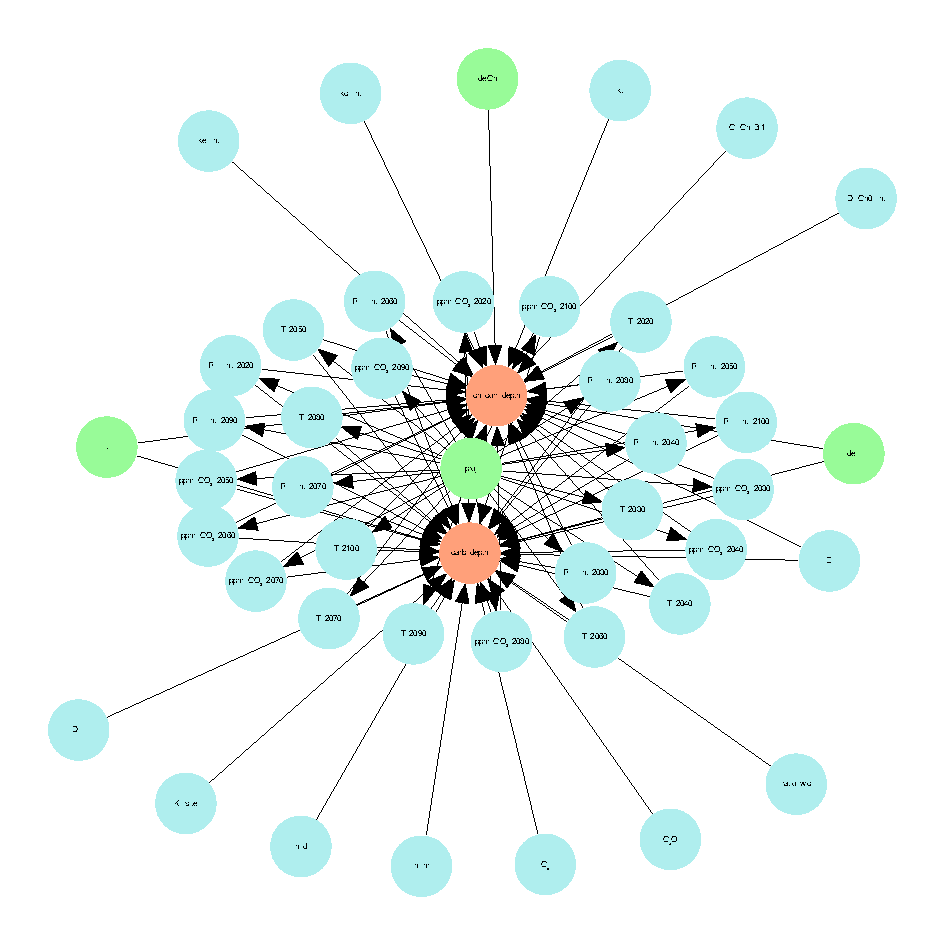
\includegraphics[width=\linewidth]{imgs/pdfs/12_total_ebn_precise.pdf}
    \caption{Concrete corrosion eBN with precise nodes}\label{fig:precise_ebn}
\end{figure}

The functional nodes \textit{ch\_corr\_depth} and \textit{carb\_depth} are initially defined through the set of continuous random variables coming from their continuous parents, the set of discrete random variables coming from their discrete parents and a simulation technique, selected to be a standard Monte Carlo with $10^4$ samples for both of them.
The union of these two sets of inputs together with the chosen simulation technique and two performance functions, allows solving the structural reliability problem. 
In this way, it is possible to obtain the two CPTs associated with the two discrete nodes \textit{ch\_corr\_depth} and \textit{carb\_depth} in the reduced BN of Fig.~\ref{fig:precise_rbn}. 

\begin{figure}[H]
    \centering
    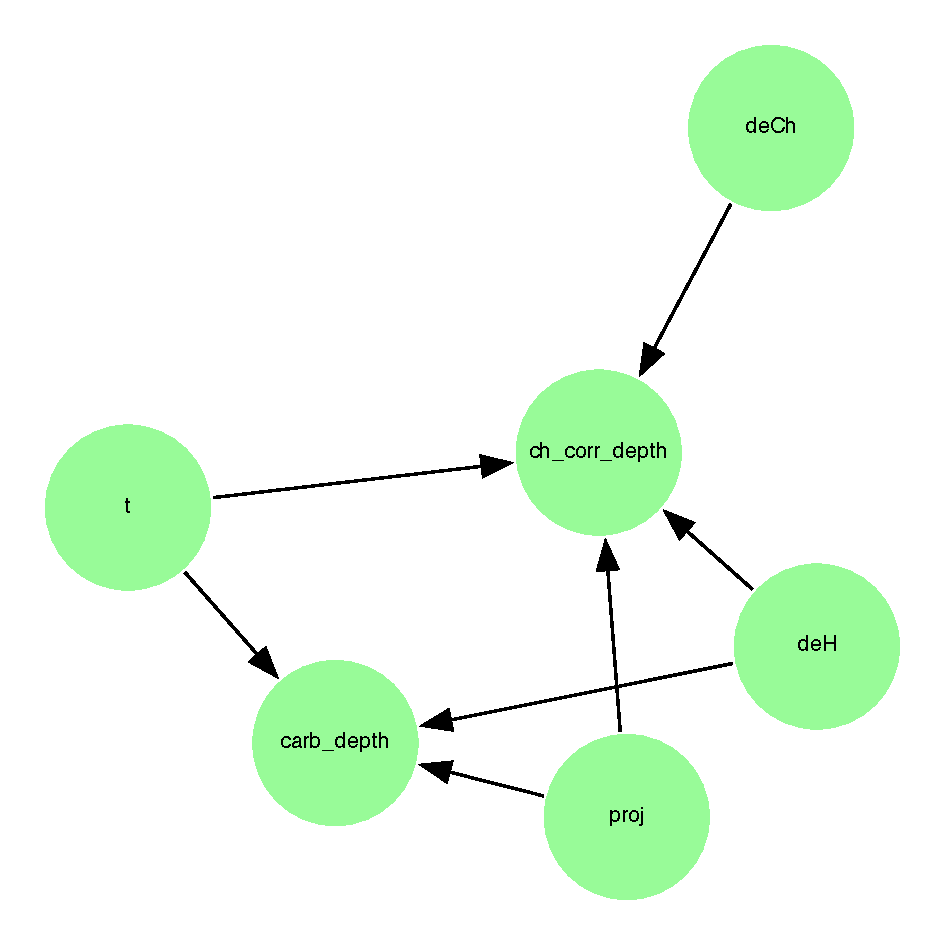
\includegraphics[scale=0.5]{imgs/pdfs/13_total_rbn_precise.pdf}
    \caption{Concrete corrosion rBN with precise nodes}\label{fig:precise_rbn}
\end{figure}

In this BN, only discrete nodes are present. Both \textit{ch\_corr\_depth} and \textit{carb\_depth} have as parents the discrete nodes referred to the specific time slice, to the specific climatic projection and the auxiliary discrete node \textit{deH}. The node \textit{deCh} influences the sole node chloride-induced corrosion process, therefore it is not a parent of \textit{carb\_depth}.

\subsubsection{Imprecise eBN -- Imprecision in climatic change data}

In the climatic change data catalogue~\cite{Copernicus_Climate_Change}, each \textit{ssp} comes from different down-scaled regional climatic models (RCMs). The Gaussian distributions defined in Tabs.~\ref{Climate_Change_Tnode_dists},~\ref{Climate_Change_RHnode_dists} and~\ref{Climate_Change_CO2node_dists} have been extrapolated based on limited number of RCMs.
A more robust way for dealing with the epistemic uncertainty problem of future projections is represented by the interval probability theory. Therefore, without introducing any hypothesis over the specific distribution, the quantities of interest have been treated as interval values, i.e.~defined only by an upper bound and a lower bound, given respectively by the maximum and minimum values of all the simulations related to a specific \textit{ssp}.

\begin{figure}[H]
    \centering
    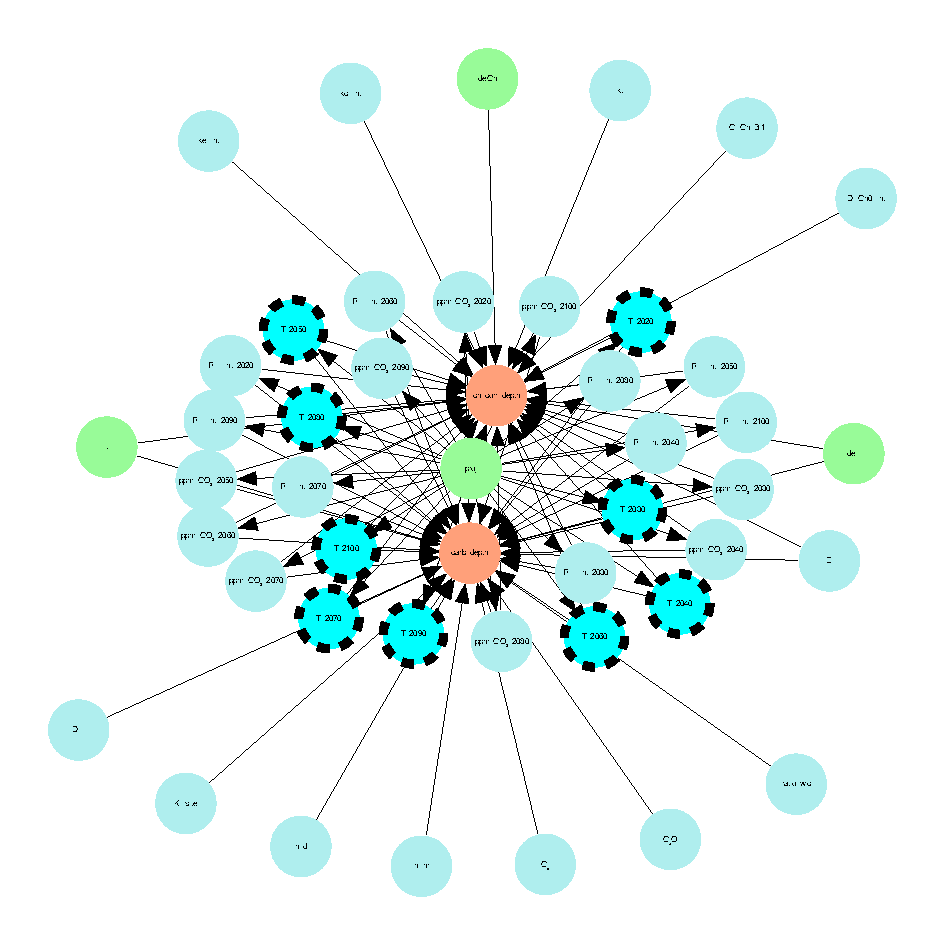
\includegraphics[width=\linewidth]{imgs/pdfs/14_total_ebn_imprecise.pdf}
    \caption{Concrete corrosion eBN with imprecise temperature nodes}\label{fig:imprecise_ebn}
\end{figure}

This concept has been applied to the temperature projections obtaining the new node presented in Fig.~\ref{fig:imprecise_ebn} and defined in Tab.~\ref{Climate_Change_Tnode_interval}. The reduced BN of this imprecise eBN is the Credal Network presented in Fig.~\ref{fig:imprecise_rbn}.
\begin{figure}[H]
    \centering
    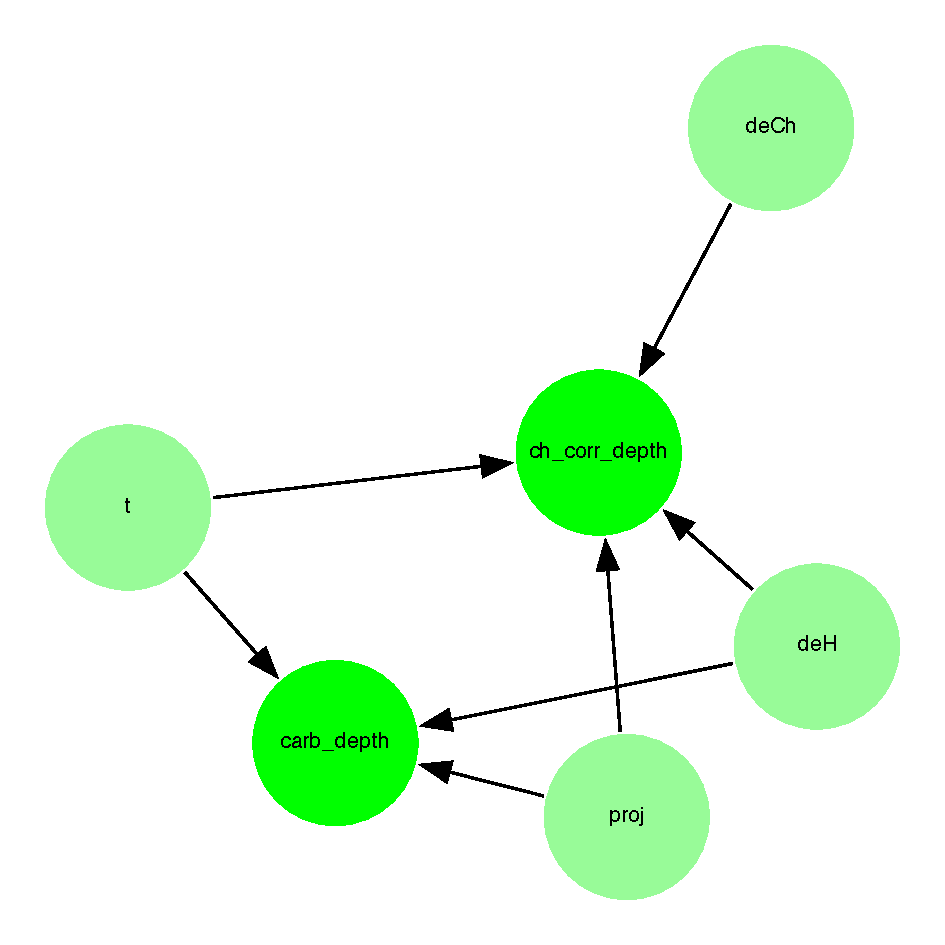
\includegraphics[scale=0.5]{imgs/pdfs/15_total_rbn_imprecise.pdf}
    \caption{Concrete corrosion risk rBN with imprecise nodes}\label{fig:imprecise_rbn}
\end{figure}